Durante l\textquoteright{}attivit\`{a} di stage sono stati riassunti i requisiti del progetto in diagrammi dei casi d\textquoteright{}uso al fine di specificare nella maniera pi\`{u} chiara e semplice possibile le specifiche per il progetto. In questa sezione viene presentato il minimo indispensabile per far comprendere il \textit{\textbf{dominio}} del progetto. Iniziando dapprima con una descrizione sullo stato del software a inizio stage e quindi prima delle operazioni di manutenzione richieste.

\subsection{Stato software a inizio stage}
Il software permette di effettuare una programmazione delle \textit{\textbf{attivit\`{a}}} inserendo per queste data di inizio, di fine e durata. La maturazione dell\textquoteright{}attivit\`{a} viene calcolata in base alla durata calcolando di default \textit{8 ore} lavorative giornaliere ed escludendo nei calcoli il sabato e le festivit\`{a}. Se una \textit{\textbf{risorsa}} viene assegnata all\textquoteright{}attivit\`{a} per un certo numero di giorni lavorativi, allora il software stabilisce che questa risorsa ha effettuato nei giorni stabiliti la stessa percentuale di ore di lavoro. Il software non considera se una risorsa \`{e} occupata in altre attivit\`{a} nella stesso periodo. Se ad una attivit\`{a} viene assegnata una risorsa con un certo numero di ore di impegno, allora per la durata dell\textquoteright{}attivit\`{a} la risorsa \`{e} stata impiegata giorno per giorno la stessa frazione di tempo.

\subsection{Casi d\textquoteright{}uso}

\subsubsection[UC1: Scenario principale]{UC1: Scenario principale}
\begin{figure}[H]
\begin{center}
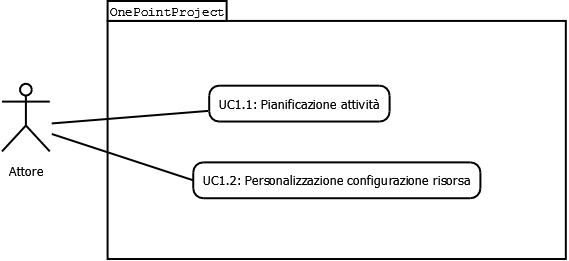
\includegraphics[width=0.80\textwidth]{img/UC/UC1.png}
\caption{UC1: Scenario principale}
\label{fig:UC1}
\end{center}
\end{figure}

\begin{description}
\item[Attori:]{utente autenticato al sistema.}
\item[Precondizione:]{Le infrastrutture di rete sono funzionanti e l\textquoteright{}applicativo \`{e} stato corretamente avviato.}
\item[Scenario principale:]{l\textquoteright{}utente pu\`{o} eseguire le seguenti operazioni:
	\begin{itemize}
	\item \textbf{pianificare le attivit\`{a}}: l\textquoteright{}utente dopo aver creato il progetto interessato o aperto in modifica uno esistente pu\`{o} utilizzare come strumento di pianificazione il \textit{\textbf{WBS}} (UC1.1);
	\item \textbf{personalizzare la configurazione di una risorsa}: l\textquoteright{}utente accedendo al pannello di amministrazione risorse pu\`{o} scegliere come configurare una risorsa in termine di costi, sia interni che esterni, e di fascie orarie di lavoro e non (UC1.2).
	\end{itemize}}
\item[Postcondizione per successo:]{il sistema \`{e} in attesa di una scelta da parte dell\textquoteright{}utente.}
\end{description}

\subsubsection[UC1.1: Pianificazione attivit\`{a}]{UC1.1: Pianificazione attivit\`{a}}
\begin{figure}[H]
\begin{center}
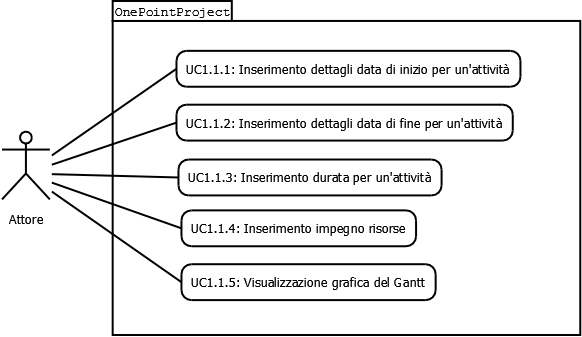
\includegraphics[width=0.80\textwidth]{img/UC/UC1.1.png}
\caption{UC1.1: Pianificazione attivit\`{a}}
\label{fig:UC1.1}
\end{center}
\end{figure}

\begin{description}
\item[Attori:]{utente autenticato al sistema.}
\item[Precondizione:]{L\textquoteright{}utente \`{e} in opzione modifica per un certo progetto e le infrastrutture di rete sono funzionanti.}
\item[Scenario principale:]{l\textquoteright{}utente pu\`{o} eseguire le seguenti operazioni:
	\begin{itemize}
	\item \textbf{inserire i dettagli relativi alla data di inizio dell\textquoteright{}attivit\`{a}}: l\textquoteright{}utente pu\`{o} inserire data e ora di inizio per un\textquoteright{}attivit\`{a} (UC1.1.1);
	\item \textbf{inserire i dettagli relativi alla data di fine dell\textquoteright{}attivit\`{a}}: l\textquoteright{}utente pu\`{o} inserire data e ora di fine per un\textquoteright{}attivit\`{a} (UC1.1.2);
	\item \textbf{inserire una durata per l\textquoteright{}attivit\`{a}}: l\textquoteright{}utente pu\`{o} inserire la durata dell\textquoteright{}attivit\`{a} nel formato dd-hh-mm che aggiorner\`{a} di conseguenza la data di fine, si tratta di un\textquoteright{}opzione alternativa all\textquoteright{}inserimento della data di fine (UC1.1.3);
	\item \textbf{inserire l\textquoteright{}impegno per le risorse coinvolte}: l\textquoteright{}utente dopo aver assegnato le risorse all\textquoteright{}attivit\`{a} interessata pu\`{o} scegliere le ore di lavoro della risorsa per l\textquoteright{}attivit\`{a} stessa (UC1.1.4);
	\item \textbf{visualizzazione del diagramma di Gantt}: l\textquoteright{}utente pu\`{o} visualizzare il diagramma di Gantt delle attivit\`{a} elencate nel WBS (UC1.1.5).
	\end{itemize}}
\item[Postcondizione per successo:]{il sistema aggiorna il WBS delle attivit\`{a} e in caso di salvataggio rende persitente la pianificazione effettuata.}
\end{description}

\subsubsection[UC1.2: Personalizzazione configurazione risorsa]{UC1.2: Personalizzazione configurazione risorsa}
\begin{figure}[H]
\begin{center}
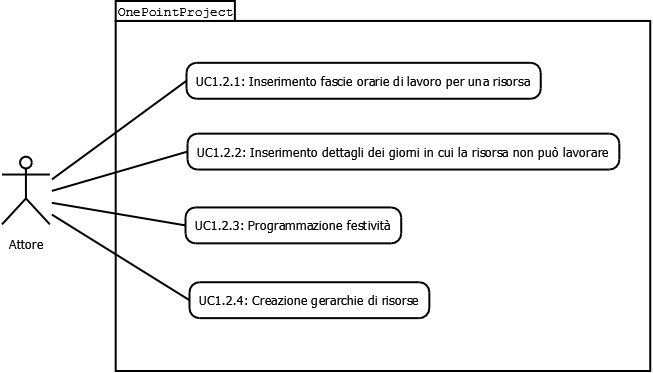
\includegraphics[width=0.80\textwidth]{img/UC/UC1.2.png}
\caption{UC1.2: Personalizzazione configurazione risorsa}
\label{fig:UC1.2}
\end{center}
\end{figure}

\begin{description}
\item[Attori:]{utente autenticato al sistema.}
\item[Precondizione:]{L\textquoteright{}utente ha i permessi per effettuare le modifiche alle risorse, ha quindi facolt\`{a} di accesso al pannello di amministrazione risorse e le infrastrutture di reste sono funzionanti.}
\item[Scenario principale:]{l\textquoteright{}utente pu\`{o} eseguire le seguenti operazioni:
	\begin{itemize}
	\item \textbf{inserire fascie orarie di lavoro per una risorsa}: l\textquoteright{}utente pu\`{o} inserire data e ora di inizio per un\textquoteright{}attivit\`{a} (UC1.2.1);
	\item \textbf{inserire i dettagli dei giorni in cui la risorsa \`{e} in stallo}: l\textquoteright{}utente pu\`{o} inserire data e facie orarie in cui la risorsa non pu\`{o} lavorare, pu\`{o} inoltre specificare le ragioni per cui la risorsa non pu\`{o} lavorare per esempio: manutenzione, locata a terzi ecc. (UC1.2.2);
	\item \textbf{programmare le festivit\`{a}}: l\textquoteright{}utente pu\`{o} indicare se una risorsa lavora o meno nei giorni festivi in base al calendario italiano (UC1.2.3);
	\item \textbf{creazione gerarchie di risorse}: l\textquoteright{}utente pu\`{o} specificare delle gerarchie di risorse tale che per una risorsa figlio \`{e} impostabile la possibilit\`{a} di ereditare o meno la configurazione del padre (UC1.2.4);
	\end{itemize}}
\item[Postcondizione per successo:]{il sistema aggiorna nel database le propriet\`{a} di configurazione delle risorse.}
\end{description}

\subsection{Lista requisiti}
Per la stesura dei requisiti \`{e} stato deciso di seguire le seguenti regole di classificazione:

\begin{doublespace}
\begin{center}
\emph{Tipo.Priorit\`{a}.(X.Y.V.W.Z)}
\par\end{center}
\end{doublespace}

Dove:
\begin{itemize}
\item \textbf{Tipo}: tipo di requisito

\begin{itemize}
\item \textbf{RF}: requisito funzionale
\end{itemize}

\item \textbf{Priorit\`{a}}: priorit\`{a} del requisito

\begin{itemize}
\item \textbf{ob}: requisito obbligatorio
\item \textbf{de}: requisito desiderabile
\item \textbf{op}: requisito opzionale
\end{itemize}
\item \textbf{X.Y.V.W.Z}: numerazione di tipo gerarchica del requisito. Ad ogni requisito diverso dovr\`{a} aumentare la numerazione X. La presenza delle
numerazioni Y, V, W e Z \`{e} opzionale. Le numerazioni di X, Y, V, W e Z partiranno da uno
\end{itemize}
Esempi: RF.ob.1.2.1, RF.de.2, RF.ob.1.2.4.2.1, ...

\subsubsection{Requisiti funzionali}
In questo paragrafo verranno elencati i principali requisiti relativi al progetto.

\subparagraph{Requisiti obbligatori} \quad \quad 

\begin{description}
\item[RF.ob.1]: Il software nell\textquoteright{}inserimento delle attivit\`{a} deve permettere l\textquoteright{}impostazione di informazioni sull\textquoteright{}inizio e sulla fine.
	\begin{description}
	\item[RF.ob.1.1]: Il software deve permettere l\textquoteright{}impostazione della data di inizio e di fine.
	\item[RF.ob.1.2]: Il software deve permettere l\textquoteright{}impostazione dell\textquoteright{}ora di inizio e di fine.
	\end{description}
\item[RF.ob.2]: Il software nell\textquoteright{}inserimento delle attivit\`{a} deve permettere l\textquoteright{}inserimento di una durata con un livello di precisione al minuto, nel formato \textit{dd-hh-mm}.
\item[RF.ob.3]: Se \`{e} stata modificata la durata e la data di fine il software deve effetture l\textquoteright{}aggiornamento della data di fine considerando la durata modificata.
\item[RF.ob.4]: Il software dovr\`{a} calcolare la data di fine partendo dalla data di inizio e sommando la durata pianificata.
	\begin{description}
	\item[RF.ob.4.1]: Il software deve calcolare il grado di avanzamento, quindi di maturazione dell\textquoteright{}attivit\`{a}, al fine di calcolare la data di fine, automaticamente.
		\begin{description}
		\item[RF.ob.4.1.1]: L\textquoteright{}ordine di calcolo deve attenersi all\textquoteright{}ordine stabilito per il WBS. 
			\begin{description}
			\item[RF.ob.4.1.1.1]: Il software deve considerare che una certa risorsa non pu\`{o} essere utilizzata se la stessa \`{e} impiegata in un\textquoteright{}altra attivit\`{a} nella stessa frazione di tempo.
			\item[RF.ob.4.1.1.2]: Il software deve considerare la disponibilit\`{a} delle risorse, cio\`{e} deve considerare il calendario configurato dall\textquoteright{}utente.
			\item[RF.ob.4.1.1.3]: Il software deve considerare che per una certa attivit\`{a} le risorse sono assegnate per una certa quantit\`{a} di ore. 
			\end{description}
		\item[RF.ob.4.1.2]: Il software dovr\`{a} considerare tipologie di calcolo diverse in relazione al tipo di risorse interessate.
			\begin{description}
			\item[RF.ob.4.1.2.1]: Il software conosce i tipi di risorsa interessati, ma non devono essere impostabili dall\textquoteright{}utente.
			\item[RF.ob.4.1.2.2]: La tipologia di risorse impiegate influenza la durata impostata sull\textquoteright{}attivit\`{a}.
				\begin{description}
				\item[RF.ob.4.1.2.2.1]: Il software se nello stesso minuto verifica la disponibilit\`{a} di pi\`{u} risorse strumentali allora il grado di maturazione dell\textquoteright{}attivit\`{a} crescer\`{a} di un minuto e l\textquoteright{}\textit{\textbf{impegno}} residuo delle risorse disponibili in quel minuto aumenter\`{a} di \textit{1 minuto}.
				\item[RF.ob.4.1.2.2.2]:Il software se nello stesso minuto verifica la disponibilit\`{a} di pi\`{u} risorse umane allora il grado di maturazione dell\textquoteright{}attivit\`{a} crescer\`{a} di un minuto e l\textquoteright{}impegno residuo delle risorse disponibili in quel minuto aumenter\`{a} della seguente quantit\`{a}: \textit{$ \log_2 n $ , con n=numero di risorse disponibili}.
				\end{description}
			\end{description}
		\item[RF.ob.4.1.3]: Il software deve effettuare l\textquoteright{}aggiornamento delle durate, ovvero il calcolo della durata delle attivit\`{a} nel momento in cui l\textquoteright{}utente decide di salvare il WBS.
		\end{description}
	\end{description}
\item[RF.ob.5]: Il software deve permettere di effettuare una configurazione delle risorse.
	\begin{description}
	\item[RF.ob.5.1]: Il software deve permettere di stabilire delle gerarchie di risorse.
		\begin{description}
		\item[RF.ob.5.1.1]: Le risorse ereditano per default le configurazioni della risorsa padre.
		\item[RF.ob.5.1.2]: Le risorse appartenenti ad una gerarchia possono non ereditare, in base alle scelte dell\textquoteright{}utente, alcune propriet\`{a} dalla risorsa padre.
		\end{description}
	\item[RF.ob.5.2]: Il software deve permettere l\textquoteright{}assegnazione delle fascie orarie in cui una certa risorsa pu\`{o} lavorare.
	\item[RF.ob.5.3]: Il software deve permettere di impostare se una certa risorsa pu\`{o} o meno lavorare nelle festivit\`{a}.
	\item[RF.ob.5.4]: Il software deve permettere di impostare le date in cui una risorsa \`{e} bloccata.
		\begin{description}
		\item[RF.ob.5.4.1]: Una risorsa pu\`{o} non essere disponibile in \textit{1 o pi\`{u}} fascie orarie della data scelta, oppure durante le \textit{24 ore} della data scelta.
		\end{description}
	\end{description}
\end{description}

\subparagraph{Requisiti desiderabili} \quad \quad 

\begin{description}
\item[RF.de.1]: Il software deve permettere la visualizzazione in ore del diagramma di Gantt.
\item[RF.de.2]: Il software deve permettere di aggiornare il WBS in relazione alle modifiche apportate al diagramma di Gantt.
\item[RF.de.3]: Il software deve permettere di effettuare modifiche sulla durata delle attivit\`{a} al diagramma di Gantt.
	\begin{description}
	\item[RF.de.3.1]: Il software deve permettere di effettuare modifiche che presentano una durata complessiva finale maggiore o uguale alla durata di un giorno.
	\item[RF.de.3.2]: Il software deve permettere di effettuare modifiche che presentano una durata complessiva finale minore alla durata di un giorno.
\end{description}
\end{description}

\subparagraph{Requisiti opzionali} \quad \quad 

\begin{description}
\item[RF.op.1]: Il software deve permettere l\textquoteright{}inserimento della percentuale di completamento delle attivit\`{a}.
\item[RF.op.2]: Il software deve permettere la colorazione delle attivit\`{a} in relazione alla percentuale di completamento.
\end{description}

